\documentclass[12pt]{article}  

\usepackage[boxruled,lined]{algorithm2e}
%% \usepackage{booktabs}
\usepackage{amsmath} 
\usepackage{amsthm} 
\usepackage{amsfonts} 
\usepackage{enumitem}
\usepackage[T1]{fontenc}
\usepackage[utf8]{inputenc}
\usepackage{xparse} 
\usepackage{bm}
\usepackage{bbm} 
\usepackage{color,soul} 
\usepackage{framed}
\usepackage[margin=0.5in]{geometry}
\usepackage{hyperref}
\usepackage{mathtools}
\usepackage{multicol}
\usepackage[dvipsnames]{xcolor}
\usepackage{tikz}
\usepackage[normalem]{ulem}
\usepackage{pgfplots}  
\usepackage{pifont}
\usetikzlibrary{positioning}
\usetikzlibrary{calc}
\usetikzlibrary{fit}
\usetikzlibrary{shapes}
\usetikzlibrary{patterns}
\usetikzlibrary{decorations.pathreplacing}
\newcommand\STAR{{\tikz{\node[draw,star,star point height=.7em,minimum size=1em,scale=0.35]{};} }}
\newcommand{\Plus}{\mathord{\begin{tikzpicture}[baseline=0ex, line width=1, scale=0.13]
\draw (1,0) -- (1,2); \draw (0,1) -- (2,1); \end{tikzpicture}}}

\newtheorem{theorem}{Theorem}[section]
\newtheorem{lemma}[theorem]{Lemma}
\newtheorem{proposition}[theorem]{Proposition}
\newtheorem{corollary}[theorem]{Corollary}
\DeclarePairedDelimiter{\ceil}{\lceil}{\rceil}
\DeclarePairedDelimiter{\floor}{\lfloor}{\rfloor}
\DeclareMathOperator*{\argmin}{arg\,min}
\DeclareMathOperator*{\argmax}{arg\,max}
\newcommand{\D}{\mathrm{d}}
\SetKwInput{KwInput}{Input}
\SetKwInput{KwOutput}{Output}

\definecolor{deepblue}{rgb}{0,0,0.5}
\definecolor{deepred}{rgb}{0.6,0,0}
\definecolor{deepgreen}{rgb}{0,0.5,0}

\usepackage{listings}

% Default fixed font does not support bold face
\DeclareFixedFont{\ttb}{T1}{txtt}{bx}{n}{12} % for bold
\DeclareFixedFont{\ttm}{T1}{txtt}{m}{n}{12}  % for normal
% Python style for highlighting
\newcommand\pythonstyle{\lstset{
language=Python,
basicstyle=\ttm,
otherkeywords={self,for,range,in},             % Add keywords here
keywordstyle=\ttb\color{deepblue},
emph={MyClass,__init__},          % Custom highlighting
emphstyle=\ttb\color{deepred},    % Custom highlighting style
stringstyle=\color{deepgreen},
frame=tb,                         % Any extra options here
showstringspaces=false            % 
}}


% Python environment
\lstnewenvironment{python}[1][]
{
\pythonstyle
\lstset{#1}
}
{}

% Python for external files
\newcommand\pythonexternal[2][]{{
\pythonstyle
\lstinputlisting[#1]{#2}}}

% Python for inline
\newcommand\pythoninline[1]{{\pythonstyle\lstinline!#1!}}


\begin{document}
\renewcommand{\d}[1]{\ensuremath{\operatorname{d}\!{#1}}}

\tableofcontents
\newpage
\section{Classification and Vector Spaces}\vspace{.1pt} \hrule height 2pt \smallskip \renewcommand{\arraystretch}{1}% Tighter
\subsection{Supervised ML and Sentiment Analysis}
In supervised ML, we have input features $X$ and a set of labels $Y$. To get the most accurate predictions, we try to minimize our \emph{error rates} or \emph{cost function} as much as possible: to do this, we'll run our prediction function which takes in parameters $\theta$ to map you input features to output labels $\hat Y$. The best mapping is achieved when the difference between the expected values $Y$ and the predicted values $\hat Y$ is minimized, which the cost function does by comparing how closely your output $\hat Y$ is to your label $Y$. You can then update your parameters and repeat the whole process until your cost is minimized.

\begin{figure}[h]
\begin{center}
  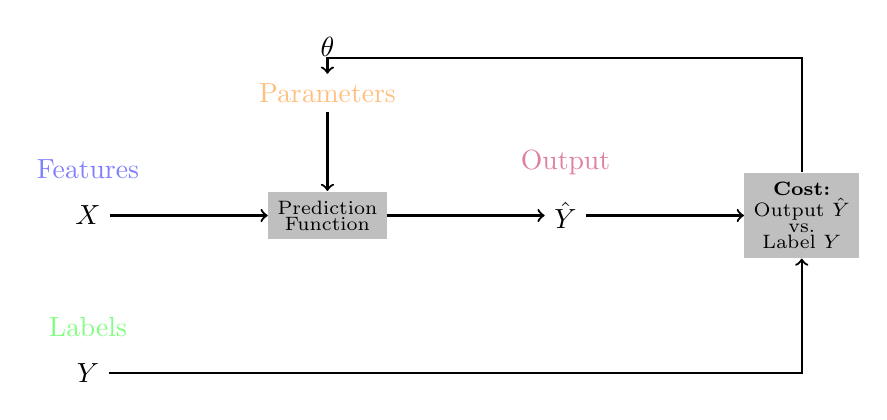
\begin{tikzpicture}
    \node (x) at (0, 2) {$X$};
    \node (features) [above=1mm of x] {\color{blue!50}{Features}};
    \node (y) at (0, 0) {$Y$};
    \node (labels) [above=1mm of y] {\color{green!50}{Labels}};
    \node[fill=gray!50,rectangle,right = 2cm of x] (predictionfunction)     {$\substack{\textrm{Prediction} \\ \textrm{Function}}$};
    \node[above = 1cm of predictionfunction] (params)     {\color{orange!50}{Parameters}};
    \node[above = 1mm of params] (theta) {$\theta$};
    \node[right = 2cm of predictionfunction] (yhat) {$\hat Y$};
    \node (output) [above=1mm of yhat] {\color{purple!50}{Output}};
    \node[fill=gray!50,rectangle,right = 2cm of yhat] (cost) {$\substack{\textrm{\textbf{Cost:}} \\ \textrm{Output } \hat Y \\ \textrm{vs.}     \\ \textrm{Label } Y}$};
\draw[->,thick] (x) -- (predictionfunction);
\draw[->,thick] (predictionfunction) -- (yhat);
\draw[->,thick] (yhat) -- (cost);
% Draw a path in two steps and go via a coordinate relative to the first node.
\draw[->,thick] (y) -- node {} ++(2cm,0) -| (cost);
\draw[->,thick] (cost) -- node{} ++(0,2cm) -| (params);
\draw[->,thick] (params) -- (predictionfunction);
\end{tikzpicture}
\end{center}
\label{fig: supervised_ml}
\caption{Overview of supervised machine learning.}
\end{figure}

How about the supervised ML classification task of sentiment analysis? Suppose we're given a tweet that says, ``I'm happy because I'm learning NLP'': and the objective in the task is to predict whether a tweet has a positive or negative sentiment. We'll do this by starting with a training set where tweets with a positive label have a label of unit value, and tweets with a negative sentiment have a label of zero.
To get started building a logistic regression classifier that's capable of predicting sentiments of an arbitrary tweet, we first need to process the raw tweets in our training data set and extract useful features. Then, we will train our logistic regression classifier while minimimizing the cost. Finally, we'll be able to make predictions.

\paragraph{How to represent text as a vector} In order to represent text as a vector, we need to first build a vocabulary. We define the vocabulary $V$ as the \emph{set} of unique words from your input data (e.g. your listing of tweets). To get this listing, we quite literally need to comb through all words from all input data and save every new word that appears in our search.
To represent a tweet as a vector, we can use a one-hot encoding with our vocabulary: i.e. each tweet will be represented with a length $|V|$ vector where elements are binary-valued - a one indicates the word is in the tweet and a zero indicates the absence of a word in a tweet. We call this a \emph{sparse} representation because the number of non-zero entries is relatively small when compared with the number of zero entries. Realize that if we are running a logistic regression, we would require learning $|V| + 1$ parameters which can be problematic for large vocabularies. If not prohibitive, it would make training models take excessive time and making predictions would be expensive.

\paragraph{Negative and positive frequencies} Let's discuss how to generate counts which can be used as features in our logistic regression classifier. Specifically, given a word, we wish to keep track of the number of times that it shows up as the positive class. Given another word, we wish to track how many times that word shows up in the negative class. Using both these counts, we can then extract features and use those features in our logistic regression classifier. Suppose we have the following corpus of tweets:
\begin{verbatim}
I am happy because I am learning NLP
I am happy
I am sad, I am not learning NLP
I am sad
\end{verbatim}
Then our vocabulary is given by
\begin{center}
  \begin{tabular}{c}
    \hline
    Vocabulary \\
    \hline
    I \\
    am \\
    happy \\
    because \\
    learning \\
    NLP \\
    sad \\
    not
  \end{tabular}
\end{center}

For this particular example of sentiment analysis, we only have two sentiments (i.e. two classes): one class is associated with a positive sentiment and the other with a negative sentiment. So, taking your corpus, you'd have a set of two tweets that belong to the positive class, and two tweets which belong to the negative class. Let's calculate the positive frequencies by examining the first two tweets:

\begin{center}
  \begin{tabular}{c c}
    \hline
    Vocabulary & PosFreq(1) \\
    \hline
    I  & 3 \\
    am & 3 \\
    happy & 2 \\
    because & 1 \\
    learning & 1 \\
    NLP & 1 \\
    sad & 0 \\
    not & 0
  \end{tabular}
\end{center}

The same logic applies applies to getting negative frequencies. We can calculate these by examining our last two training examples.


\begin{center}
  \begin{tabular}{c c}
    \hline
    Vocabulary & NegFreq(0) \\
    \hline
    I  & 3 \\
    am & 3 \\
    happy & 0 \\
    because & 0 \\
    learning & 1 \\
    NLP & 1 \\
    sad & 2 \\
    not & 1
  \end{tabular}
\end{center}

So, we can now have an entire table for our corpus, where for each entry in $V$ we associate with it a scalar value \texttt{PosFreq(1)} and another scalar value \texttt{NegFreq(0)}. In practice, we use a Python dictionary \texttt{freqs} mapping from \texttt{(word, class)} $\leadsto$ frequency.

\paragraph{Feature extraction with frequencies} Whereas we previously learned to encode a tweet as a vector of length $|V|$, we will now use our frequency counts to represent each tweet as a vector of length equal to one plus the number of classes in our set of labels. This gives us a much faster speed for our logistic regression classifier. How can we do this, exactly? We represent each tweet as follows:

\begin{align*}
\underbrace{X_m}_{\substack{\textrm{Features of} \\ \textrm{tweet } m}} = \bigg [ \underbrace{1}_{\textrm{Bias}}, \underbrace{\sum_w \texttt{freqs}(w, 1)}_{\substack{\textrm{Sum Pos.} \\ \textrm{Frequences}}}, \underbrace{\sum_w \texttt{freqs}(w, 0)}_{\substack{\textrm{Sum Neg.} \\ \textrm{Frequencies}}} \bigg ]
\end{align*}

I.e. the first feature is a bias unit equal to unit value, the second is the sum of positive frequencies for every unique word on tweet $m$, and the third is the sum of negative frequencies for every unique word on the tweet.
So, to extract the features for this \emph{representation}, we only have to sum frequencies of words, which is straightforward. Let's look at an example: ``I am sad, I am not learning NLP''. The only words in our vocabulary that don't appear in this sentence are ``happy'' and ``because'': if we sum up the \texttt{PosFreq(1)} associated with the remaining words in our vocabulary, i.e. the words that appear in this tweet, we get a scalar value of eight. We do the same for the negative frequencies, and we get a scalar value of eleven. So, we represent ``I am sad, I am not learning NLP'' $\leadsto [1, 8, 11]$.

\paragraph{Preprocessing} There are two major concepts here: stemming and ``stop words''. We'll learn how to apply these preprocessing steps to our data. Stop words are defined as those which don't add significant meaning to the tweets; we \emph{might} also choose to remove punctuation (if we decide it doesn't provide information in our context). In practice, this means comparing our tweet against two sets: one with stop words (in English) and another with punctuation. 

\begin{minipage}{1.0\textwidth}
  \begin{multicols}{2}
      \begin{tabular}{c c}
        \hline
        Stop Words \\
        \hline
        and \\
        is \\
        are \\
        at \\
        has \\
        for \\
        a \\
      \end{tabular}
    \vfill\null \columnbreak  
    \begin{tabular}{c c}
      \hline
      Punctuation \\
      \hline
      , \\
      . \\
      : \\
      ! \\
      `` \\
      ' \\
    \end{tabular}
\end{multicols}
\end{minipage}
In practice the list of stop words and punctuation marks are much larger, but for pedagogical purposes these will serve well.
We might start out with a tweet like
\begin{verbatim}
@YMourri and @AndrewYNg are tuning a GREAT AI Model at https://deeplearning.ai!!!
\end{verbatim}
We then preprocess by stripping stop words ``and'', ``are'', a''at'', and ``a''. The only punctuation that appears in this tweet that's also in our list is the exclamation point(s). We might further decide that tweets should have handles and URLs removed, because these don't add value for the specific task of sentiment analysis. In the end, we end up with a data point that looks like
\begin{verbatim}
tuning GREAT AI model
\end{verbatim}
It's clearly a positive tweet, and a sufficiently good model should be able to classify it. Now that the tweet contains the minimum necessary information, we can perform \emph{stemming} for every word.

\paragraph{Stemming}
Stemming in NLP is simply transforming any word to its base stem, which you could define as the set of characters that are used to construct the words and its derivatives. Let's look at the first word in the example: its stem is ``tun'', since
\begin{center}
  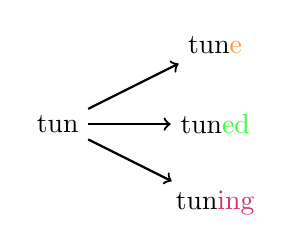
\begin{tikzpicture}
    \node (tun) at (-1,0) {tun};
    \node (tune) at (1, 1) {tun\color{orange!80}{e}};
    \node (tuned) at (1, 0) {tun\color{green!80}{ed}};
    \node (tuning) at (1, -1) {tun\color{purple!80}{ing}};
    \draw[->,thick] (tun) -> (tune);
    \draw[->,thick] (tun) -> (tuned);
    \draw[->,thick] (tun) -> (tuning);
  \end{tikzpicture}
\end{center}

If we were to perform stemming on our entire corpus, the words ``tune'', ``tuned'', and ``tuning'' all get reduced to the stem ``tun''. So, your vocabulary would be significantly reduced in performing this process. You can further reduce the size of the vocabulary without losing valuable information by \emph{lower-casing} every word, e.g. the words ``GREAT'', ``Great'', and ``great'' all get treated as the same word. Perhaps our final preprocessed tweet looks like
\begin{verbatim}
[tun, great, ai, model]
\end{verbatim}

In summary, for our example of sentiment analysis on tweets, we might preprocess as follows:
\begin{enumerate}
\item Eliminate handles and URLs
\item Tokenize the string into words
\item Remove stop words like ``and, is, a, on, etc.''
\item Stemming - or convert every word to its stem. E.g. dancer, dancing,   danced, becomes ``danc''. You can use \href{https://tartarus.org/martin/PorterStemmer/}{Porter Stemmer} to take care of this.
\item Convert all words to lowercase.
\end{enumerate}

As an applied example:
$$
\textrm{I am Happy Because I am learning NLP @deeplearning} \overset{\small \textrm{Preprocessing}}{\longrightarrow} [\texttt{happy, learn, nlp}] \overset{\small \textrm{Feature Extraction}}{\longrightarrow} [1, 4, 2]
$$
where 1 is our bias term, 4 is the sum of positive frequencies, and 2 is the sum of negative frequencies.
In practice, we are given a set of $m$ raw tweets, and so wehave to process them one-by-one to process them into an $m \times 3$ matrix, where each row describes the features for a given tweet.

\begin{equation*}
  \begin{bmatrix}
    1 & X_1^{(1)} & X_2^{(1)} \\
    1 & X_1^{(2)} & X_2^{(2)} \\
    \vdots & \vdots & \vdots \\
    1 & X_1^{(m)} & X_2^{(m)} \\
  \end{bmatrix}
\end{equation*}

The process is simple: (i) build the frequencies dictionary, (ii) initialize the matrix $X$ to match the number of tweets, (iii) go through your sets of tweets and carefully preprocess by deleting stop words, stemming, deleting URLs/handles, and lowercasing, and finally (iv) extract the features by summing up the positive and negative frequencies of each of the tweets.

\begin{python}
freqs = build_freqs(tweets, labels)          # Build frequencies dictionary.
X = np.zeros((m,3))                          # Initialize matrix X.
for i in range(m):                           # For every tweet:
  p_tweet = process_tweet(tweets[i])         #   Process tweet.
  X[i,:] = extract_features(p_tweet, freqs)  #   Extract features.
\end{python}

\subsection{Logistic Regression} Previously, we've learned how to extract features, which we will now use to predict whether a tweet has a positive or negative sentiment. Logistic regression makes use of a \href{https://en.wikipedia.org/wiki/Logistic_function#Mathematical_properties}{sigmoid (or standard logistic) function} which outputs a probability between zero and one. What's the recap from supervised machine learning? Recall figure \ref{fig: supervised_ml}: in the case of logistic regression our prediction function is going to be the standard logistic function:

\[
  h(x^{(i)}, \theta) = \frac{1}{1 + e^{-\theta^T x^{(i)}}}.
\]
where $i$ denotes the observation number. Note that as $\theta^T x^{(i)}$ gets closer and closer to $-\infty$, the denominator of the sigmoid expression blows up and as a result the output values gets closer to zero. Conversely, as the inner product $\theta^T x^{(i)}$ gets closer to $\infty$, the denominator of the sigmoid function approaches unit value and the resulting sigmoid expression evaluates to something near one.
For classification, a threshold is needed, and it is natural to set it at $\frac{1}{2}$. For the logistic function, this threshold occurs when the inner product $\theta^T x^{(i)} = 0$. If the inner product is greater than (or equal to) zero, we classify as positive, else negative.

\paragraph{How to learn $\theta$?} To train a logistic regression classifier, we need to iterate until we find a set of parameters $\theta$ that minimizes our cost function. Suppose we have a loss that depends only on the parameters $\theta_1, \theta_2$: you might have a cost function that looks like follows, on the left, with the evaluation of the cost function plotted on the right as a function of the number of training iterations:

\begin{minipage}{1.0\textwidth}
  \begin{multicols}{2}
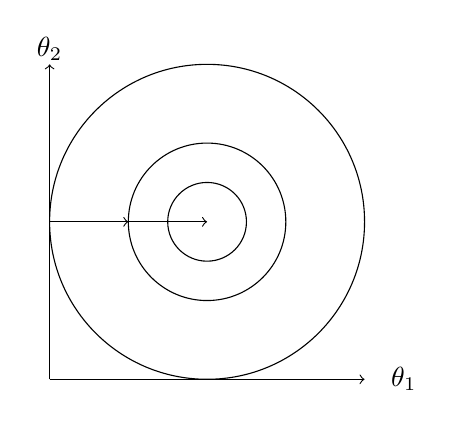
\begin{tikzpicture}[scale=2]
  \draw[->] (-1, -1) to (-1, 1);
  \node at (-1, 1.1) {$\theta_2$};
  \draw[->] (-1, -1) to (1, -1);
  \node at (1.25, -1) {$\theta_1$};
  \draw (0, 0) circle (1cm);   
  \draw (0, 0) circle (.5cm); 
  \draw (0, 0) circle (.25cm); 
  \draw[->] (-1, 0) to (-.5, 0);
  \draw[->] (-.5, 0) to (0, 0);
\end{tikzpicture}
\vfill\null \columnbreak
\begin{tikzpicture}[scale=3]
  \draw[->] (0, 0) to (0, 1.4) node [left] {cost};
  \draw[->] (0, 0) to (2.1, 0) node [right]{\# iterations}; 
  \draw[smooth, domain=0.2:2, color=orange, thick]
    plot (\x,{exp(-\x)}) {};
\end{tikzpicture}
\end{multicols}
\end{minipage}

We might first initialize our parameters $\theta$, then update our parameters in the direction of the \emph{gradient of the cost function}. After a sufficient number of training steps, we will have updated $\theta$ to their optimal values where we are achieving near optimal cost. Let's quickly review this process of gradient descent for logistic regression:

\begin{figure}[h]
\begin{center}
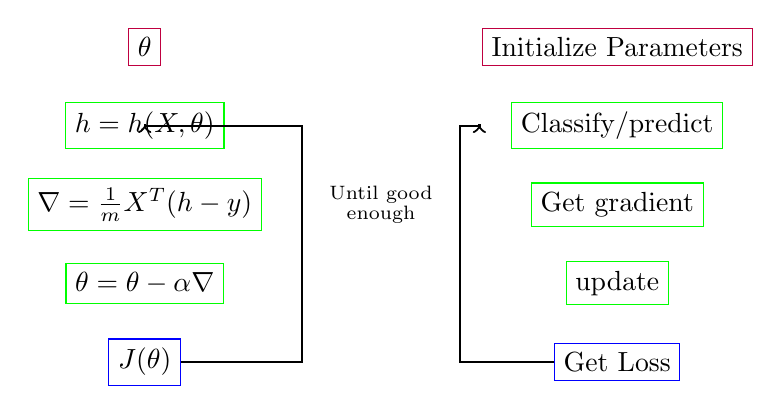
\begin{tikzpicture}
  % Left partition
  \node[draw,rectangle,color=purple] (theta) at (-2, 2) {\color{black}$\theta$};
  \node[draw,rectangle,color=green] (h) at (-2, 1) {\color{black}$h = h(X,\theta)$};
  \node[draw,rectangle,color=green] (gradient) at (-2, 0) {\color{black}$\nabla = \frac{1}{m} X^T (h-y)$};
  \node[draw,rectangle,color=green] (update_eq) at (-2, -1) {\color{black}$\theta = \theta - \alpha \nabla$};
  \node[draw,rectangle,color=blue] (cost) at (-2, -2)   {\color{black}$J(\theta)$};
  \draw[->,thick] (cost) -- ++(2, 0) -- ++(0,3) -| (h);
  % Right partition
  \node[draw,rectangle,color=purple] (init) at (4, 2) {\color{black}Initialize Parameters};
  \node[draw,rectangle,color=green] (classifypredict) at (4, 1) {\color{black}Classify/predict};
  \node[draw,rectangle,color=green] (gradient) at (4, 0) {\color{black}Get gradient};
  \node[draw,rectangle,color=green] (update_eq) at (4, -1) {\color{black}update};
  \node[draw,rectangle,color=blue] (getloss) at (4, -2)   {\color{black}Get Loss};
\draw[->,thick] (getloss) -- ++(-2, 0) -- ++(0,3) -| ++(0.25, 0);

% Middle comment
\node at (1, 0) {$\substack{\textrm{Until good} \\ \textrm{enough}}$};
\end{tikzpicture}
\end{center}
\end{figure}

\paragraph{Analyzing whether a model generalizes well}
To analyze model fit, we need the following: $(X_{\textrm{val}}, Y_{\textrm{val}}, \theta)$, where we have \emph{validation} data that was set aside during training, and a learned $\theta$ parameter vector. We will compute, for each example in $X_{\textrm{val}}$, the value of $h(\theta, x^{(i)})$ and compare it with our threshold value to make a prediction. In particular, our simple prediction function is given by
\[
  \hat Y_{\textrm{val}} = h(X_{\textrm{val}}, \theta) \geq \frac{1}{2}.
\]

In particular, we will have a vector $h = \begin{bmatrix} h_1 & h_2 & \ldots & h_m \end{bmatrix}$ where e.g. $h_i$ could equal some float in $[0,1]$, which we then convert into a binary label vector by applying our threshold. After building our predictions vector $\hat Y_{\textrm{val}}$, we can compare the predictions with the actual values and evaluate our test-set \emph{accuracy}:

\begin{equation*}
\texttt{Accuracy} = \sum_{i=1}^m \frac{\left(\texttt{pred}^{(i)} == \hat Y_{\textrm{val}}^{(i)}\right)}{m}.
\end{equation*}

This metric gives an estimate of the number of times of logistic regression model will work correctly on unseen data.

\paragraph{Logistic regression: cost function} Let's examine the equation for the cost function for logistic regression:

\begin{equation}
  \label{eq: crossentropyloss}
  J(\theta) = -\frac{1}{m} \sum_{i=1}^{m} \left[ y^{(i)} \log h(x^{(i)}, \theta) + (1 - y^{(i)}) \log \left(1 - h(x^{(i)}, \theta)\right)\right].
\end{equation}

The deep learning notes derive this equation in detail in the introduction. Let us briefly recap.
\[
  \Pr(y | x^{(i)}, \theta) = h(x^{(i)}, \theta)y^{(i)}\left(1 - h(x^{(i)}, \theta)\right)^{(1-y^{(i)})}.
\]

We wish to maximize our function $h(\cdot, \theta)$ over the parameter space $\theta$: when $y=0$ we want $(1 - h(x^{(i)}, \theta))$ to be zero, and therefore $h(x^{(i)}, \theta)$ close to one. When $y=1$, we want $h(x^{(i)},\theta) = 1$. To model our entire dataset and not just one observation, we make an assumption of independence to arrive at a joint likelihood:
\[
  L(\theta) = \prod_{i=1}^m h(x^{(i)}, \theta)^{y^{(i)}} \left(1 - h(x^{(i)}, \theta)\right)^{(1 - y^{(i)})}.
\]

Realize that if we ``mess up'' one prediction, we have the potential to ``mess up'' the entire cost function, which is what we want: we want a model that captures the entire dataset, where all datapoints are related. One issue: what happens when $m$ grows? Then $L(\theta) \leadsto 0$, because the expressions
$h(x^{(i)}, \theta)$ and correspondingly $(1 - h(x^{(i)}, \theta)$ are bounded between $(0,1)$. Using properties of logarithms (that they are monotone and maximizing a function under a monotone transformation doesn't change the optimum, and that they turn multiplication into addition), i.e.
\begin{align*}
  \log(a*b*c) = \log a + \log b + \log c \, \, \, \, \, \textrm{ and } \, \, \, \, \, \log a^b = b \log a.
\end{align*}
We may now rewrite our optimization problem:
\begin{align*}
  \max_{h(x^{(i)}, \theta)} \log L(\theta) &= \log \prod_{i=1}^{m} h(x^{(i)},                                              \theta)^{y^{(i)}} \left(1 - h(x^{(i)}, \theta)\right)^{1 - y^{(i)}} \\
  &= \sum_{i=1}^{m} \log h(x^{(i)}, \theta)^{y^{(i)}} \left(1 - h(x^{(i)},     \theta)\right)^{1 - y^{(i)}} \\
  &= \sum_{i=1}^{m} \log h(x^{(i)}, \theta)^{y^{(i)}}  + \log \left(1 - h(x^{(i)}, \theta)\right)^{1 - y^{(i)}} \\
  &= \sum_{i=1}^{m} y^{(i)} \log h(x^{(i)}, \theta) + (1 - y^{(i)}) \log \left(1 - h(x^{(i)}, \theta)\right)  
\end{align*}

We can then rescale by $\frac{1}{m}$ to get \emph{average} cost. Recall we are maximizing over $h(x^{(i)}, \theta)$ in the equation above, and maximizing an equation is the same as minimizing its negative. Therefore,
\[
  J(\theta) = -\frac{1}{m} \sum_{i=1}^{m} \left[ y^{(i)} \log h(x^{(i)}, \theta) + (1 - y^{(i)}) \log \left(1 - h(x^{(i)}, \theta)\right)\right]. 
\]

A vectorized implementation is given by
\begin{align*}
  h &= g(X\theta) \\
  J(\theta) &= \frac{1}{m} \cdot \left(-y^T \log(h) - \left(1 - y \right)^T \log (1 - h)\right)
\end{align*}

Now, let's just go over some intuition here. Consider the term on the left-hand side of the parenthesized expression: this is the relevant term in your cost function when your label is 1. The term on the right is relevant when the label is zero. In general, this loss function simply says: the closer the prediction is to the observed label, the smaller the loss incurred. We can plot the cost as a function of our the prediction value for a single training example.

\begin{minipage}{1.0\textwidth}
  \begin{multicols}{2}
    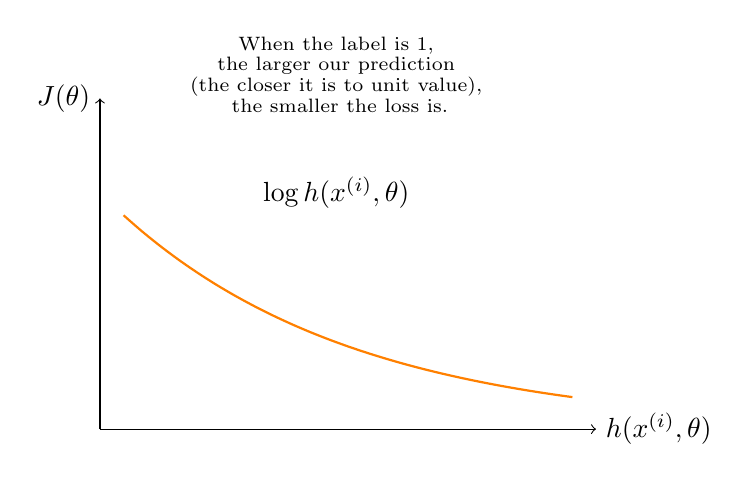
\begin{tikzpicture}[scale=3]
      \draw[->] (0, 0) to (0, 1.4) node [left] {$J(\theta)$};
      \draw[->] (0, 0) to (2.1, 0) node [right]{$h(x^{(i)}, \theta)$}; 
      \draw[smooth, domain=0.1:2, color=orange, thick]
      plot (\x,{exp(-\x)}) {};
      % plot (\x,{-log2(\x/2)}) {};
      \node at (1, 1) {$\log h(x^{(i)}, \theta)$};
      \node at (1, 1.5) {$\substack{\textrm{When the label is 1,} \\ \textrm{the larger our prediction} \\ \textrm{(the closer it is to unit value),} \\ \textrm{ the smaller the loss is.}}$};
    \end{tikzpicture}
    \vfill\null \columnbreak
    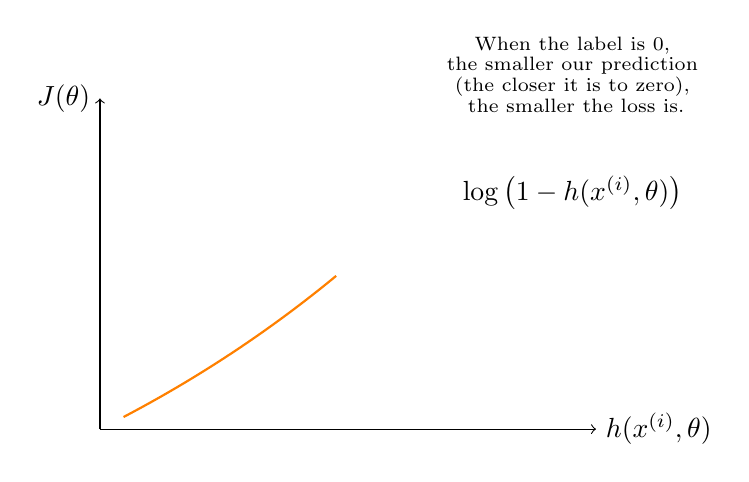
\begin{tikzpicture}[scale=3]
      \draw[->] (0, 0) to (0, 1.4) node [left] {$J(\theta)$};
      \draw[->] (0, 0) to (2.1, 0) node [right]{$h(x^{(i)}, \theta)$}; 
      \draw[smooth, domain=0.1:1, color=orange, thick]
      % plot (\x,{\x^2}) {};
      plot (\x, {exp(\x/2)-1}) {};
      \node at (2, 1) {$\log \left(1 -  h(x^{(i)}, \theta)\right)$};
      \node at (2, 1.5) {$\substack{\textrm{When the label is 0,} \\ \textrm{the smaller our prediction} \\ \textrm{(the closer it is to zero),} \\ \textrm{ the smaller the loss is.}}$};    \end{tikzpicture}
  \end{multicols}
\end{minipage}

\paragraph{Deriving logistic regression gradient}
The general form of logistic regression is given by
\begin{algorithm}
  \caption{General form of gradient descent}
  \While{not converged, and for all $j$}{
    $\theta_j \gets \theta_j - \alpha \frac{\partial}{\partial \theta_j}     J(\theta)$
  }
\end{algorithm}
We can work out the derivative using partial calculus to fill in the expression further:
\begin{algorithm}
  \caption{Gradient descent for logistic regression}
  \While{not converged, and for all $j$}{
    $\theta_j \gets \theta_j - \frac{\alpha}{m} \sum_{i=1}^m \left(h(x^{(i)}, \theta) - y^{(i)}\right) x_j^{(i)}$
  }
\end{algorithm}

A vectorized implementation is given by
\[
  \theta := \theta - \frac{\alpha}{m} X^T \left(H(X,\theta) - Y\right).
\]

\paragraph{Partial derivative of $J(\theta)$} It'll be helpful to first calculate the derivative of the sigmoid function.
\begin{align*}
  h(x)' &= \left( \frac{1}{1 + e^{-x}} \right)' = \frac{-(1 + e^{-x})'}{(1 + e^{-x})^2} = \frac{-1' - (e^{-x})'}{(1 + e^{-x})^2} = \frac{0 -           (-x)'(e^{-x})}{(1 + e^{-x})^2} = \frac{e^{-x}}{(1 + e^{-x})^2} \\
        &= \left( \frac{1}{1 + e^{-x}} \right) \left( \frac{e^{-x}}{1 + e^{-x}} \right) = h(x) \left( \frac{+1 - 1 + e^{-x}}{1 + e^{-x}} \right) = h(x) \left(\frac{1+e^{-x}}{1+e^{-x}} - \frac{1}{1+e^{-x}}\right) = h(x) (1 - h(x)).
\end{align*}

The above was all for a computation of the derivative of the sigmoid function. But what about the derivative of $h(x^{(i)}, \theta) = \frac{1}{1 + e^{-\theta^T x^{(i)}}}$ with respect to $\theta_j$? Using the chain rule, because of the inner product $\theta^T x^{(i)}$, and applying toward $\theta_j$, we see that the derivative would be
\[
  h(x^{(i)},\theta)\left(1 - h(x^{(i)},\theta)\right) x_j^{(i)}.
\]

Now, we can compute the partial derivative of our loss function with respect to $\theta_j$:

\begin{align*}\frac{\partial}{\partial \theta_j} J(\theta) &= \frac{\partial}{\partial \theta_j} \frac{-1}{m}\sum_{i=1}^m \left [ y^{(i)} log ( h(x^{(i)}, \theta) ) + (1-y^{(i)}) log (1 -  h(x^{(i)}, \theta)) \right ] \\ &= - \frac{1}{m}\sum_{i=1}^m \left [     y^{(i)} \frac{\partial}{\partial \theta_j} log ( h(x^{(i)}, \theta))   + (1-y^{(i)}) \frac{\partial}{\partial                                                                                  \theta_j} log (1 -  h(x^{(i)}, \theta))\right ] \\
                                                           &= - \frac{1}{m}\sum_{i=1}^m \left [     \frac{y^{(i)} \frac{\partial}{\partial \theta_j}  h(x^{(i)}, \theta)}{ h(x^{(i)}, \theta)}   + \frac{(1-y^{(i)})\frac{\partial}{\partial                                                      \theta_j} (1 -  h(x^{(i)}, \theta))}{1 -  h(x^{(i)}, \theta)}\right ] \\
                                                           &= - \frac{1}{m}\sum_{i=1}^m \left [     \frac{y^{(i)} \frac{\partial}{\partial \theta_j}  h(x^{(i)}, \theta)}{ h(x^{(i)}, \theta)}   + \frac{(1-y^{(i)})\frac{\partial}{\partial \theta_j} (1 -  h(x^{(i)}, \theta))}{1                                                              -  h(x^{(i)}, \theta)}\right ] \\
                                                           &= - \frac{1}{m}\sum_{i=1}^m \left [     \frac{y^{(i)}  h(x^{(i)}, \theta) (1 -  h(x^{(i)}, \theta)) \frac{\partial}{\partial \theta_j} \theta^T x^{(i)}}{ h(x^{(i)}, \theta)}   + \frac{- (1-y^{(i)})  h(x^{(i)}, \theta)(1 -  h(x^{(i)}, \theta)) \frac{\partial}{\partial \theta_j} \theta^T x^{(i)}}{1 -  h(x^{(i)},                                                              \theta)}\right ] \\
                                                           &= - \frac{1}{m}\sum_{i=1}^m \left [     \frac{y^{(i)}  h(x^{(i)}, \theta) (1 -  h(x^{(i)}, \theta)) \frac{\partial}{\partial \theta_j} \theta^T x^{(i)}}{ h(x^{(i)}, \theta)}   - \frac{(1-y^{(i)}) h(x^{(i)}, \theta) (1 -  h(x^{(i)}, \theta)) \frac{\partial}{\partial \theta_j} \theta^T x^{(i)}}{1 -  h(x^{(i)},                                                              \theta))}\right ] \\
                                                           &= - \frac{1}{m}\sum_{i=1}^m \left [     y^{(i)} (1 -  h(x^{(i)}, \theta)) x^{(i)}_j                                                              - (1-y^{(i)})  h(x^{(i)}, \theta) x^{(i)}_j\right ] \\
                                                           &= - \frac{1}{m}\sum_{i=1}^m \left [     y^{(i)} (1 -  h(x^{(i)}, \theta)) -                                                              (1-y^{(i)})  h(x^{(i)}, \theta) \right ] x^{(i)}_j \\
                                                           &= - \frac{1}{m}\sum_{i=1}^m \left [     y^{(i)} - y^{(i)}  h(x^{(i)}, \theta) -                                                               h(x^{(i)}, \theta) + y^{(i)}  h(x^{(i)}, \theta) \right ] x^{(i)}_j \\
                                                           &= - \frac{1}{m}\sum_{i=1}^m \left [ y^{(i)} -  h(x^{(i)}, \theta) \right ] x^{(i)}_j    \\
                                                           &= \frac{1}{m}\sum_{i=1}^m \left [  h(x^{(i)},                               \theta) - y^{(i)} \right ] x^{(i)}_j
\end{align*}
The vectorized version is simply given by
\[
  \nabla J(\theta) = \frac{1}{m} \cdot X^T \left( H(X, \theta) - Y \right).
\]
\end{document}

